\documentclass[a4paper,12pt]{article}

\usepackage{../usfdvl}


\title{Worksheet 11}
\SetDocumentFooter{}{}


\begin{document}

\maketitle

\worksheetGroundRules

\worksheetSubmission

\assignmentInstructions

For the following point set, find the Voronoi diagram using the insertion method. Show the algorithm using the following pages. Be sure to show all of the steps and the order of steps for the algorithm (i.e., all of the intersections).

\begin{itemize}

\item Use each steps to determine the best/average/worst case big-O performance for a single iteration. 
\item Combine that information to determine the best/average/worst case big-O for the entire computation.

\end{itemize}


\begin{center}
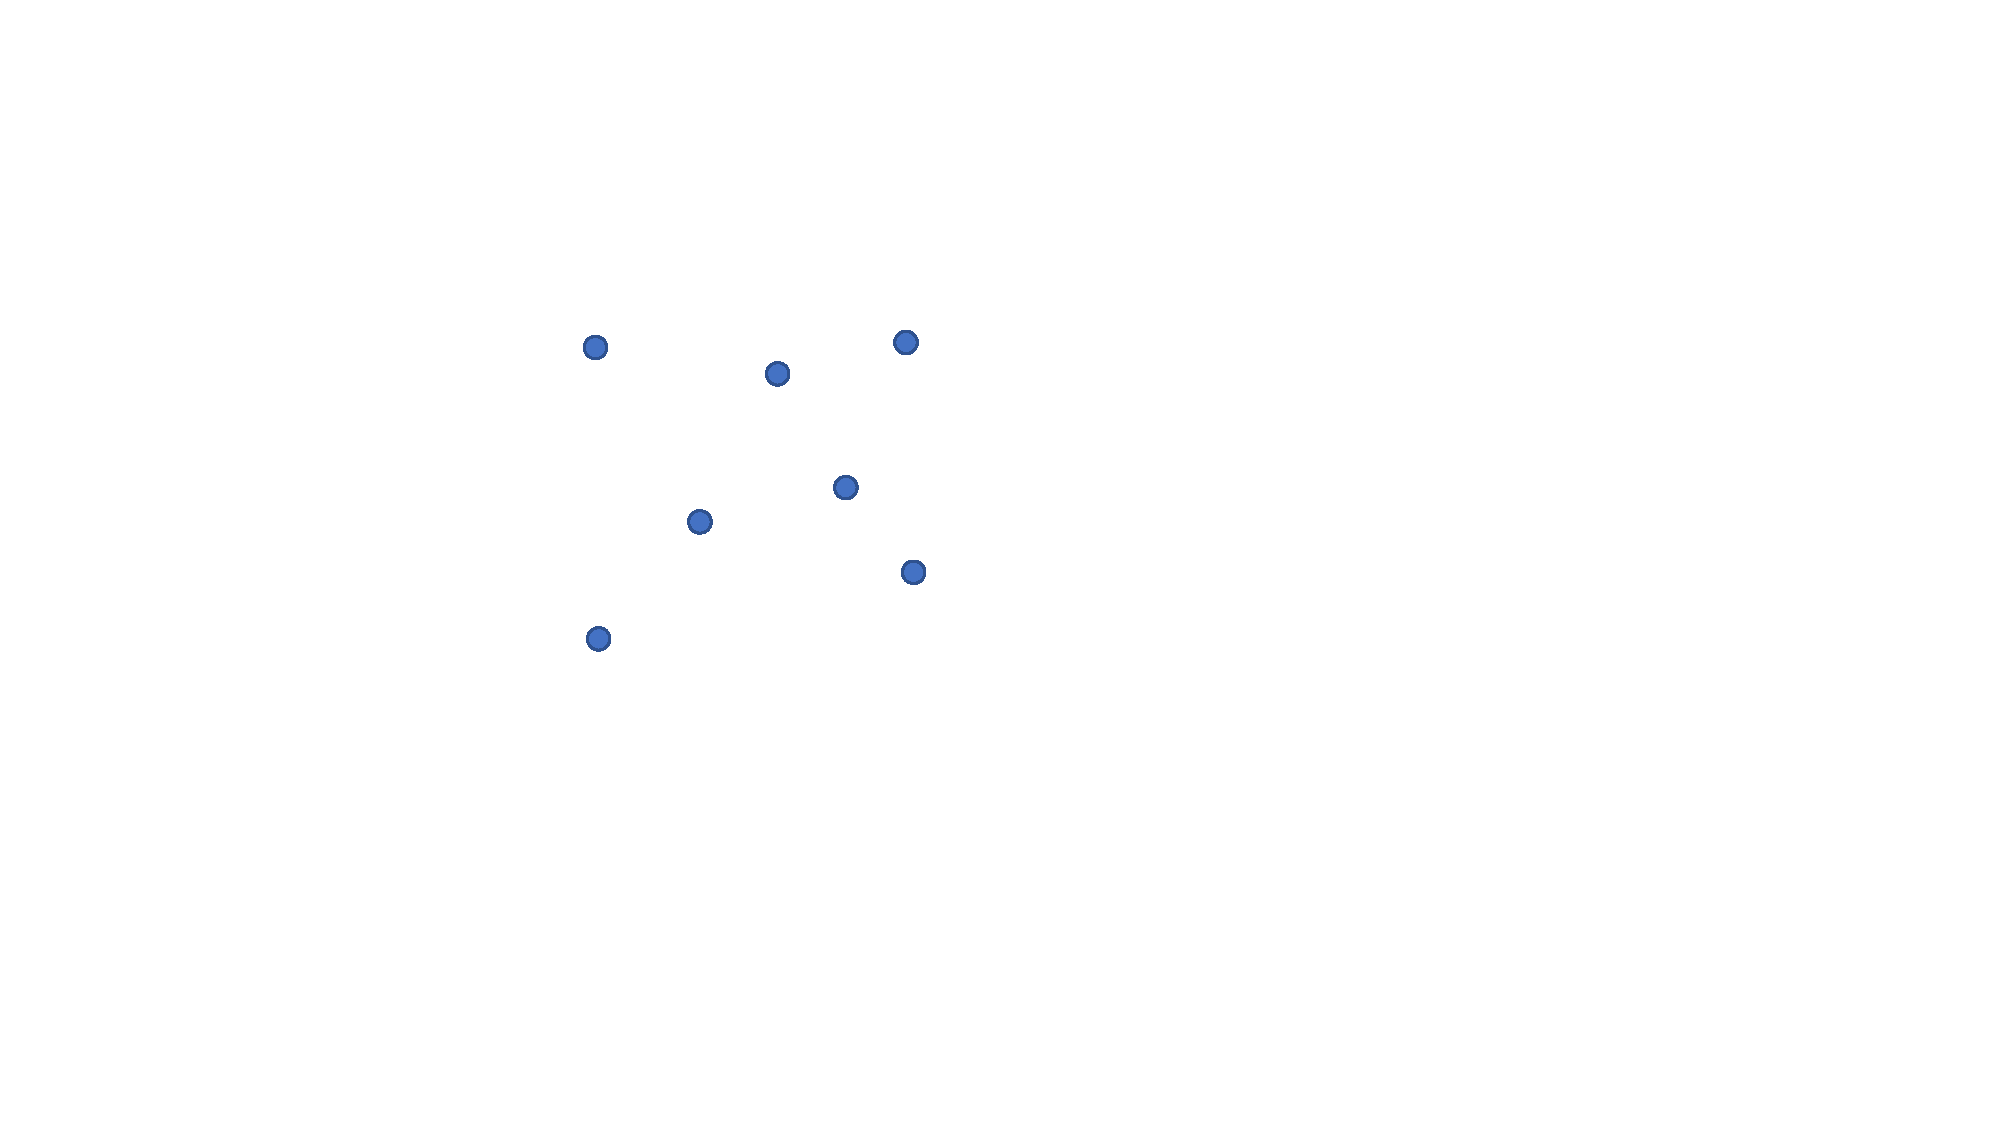
\includegraphics[width=0.65\linewidth]{../images/voronoi7.pdf}
\end{center}




\newpage

\begin{tabular}{|c|c|}
\hline
\hspace{10pt}
\includegraphics[width=0.425\linewidth]{../images/voronoi1.pdf}\hspace{10pt} & \hspace{10pt}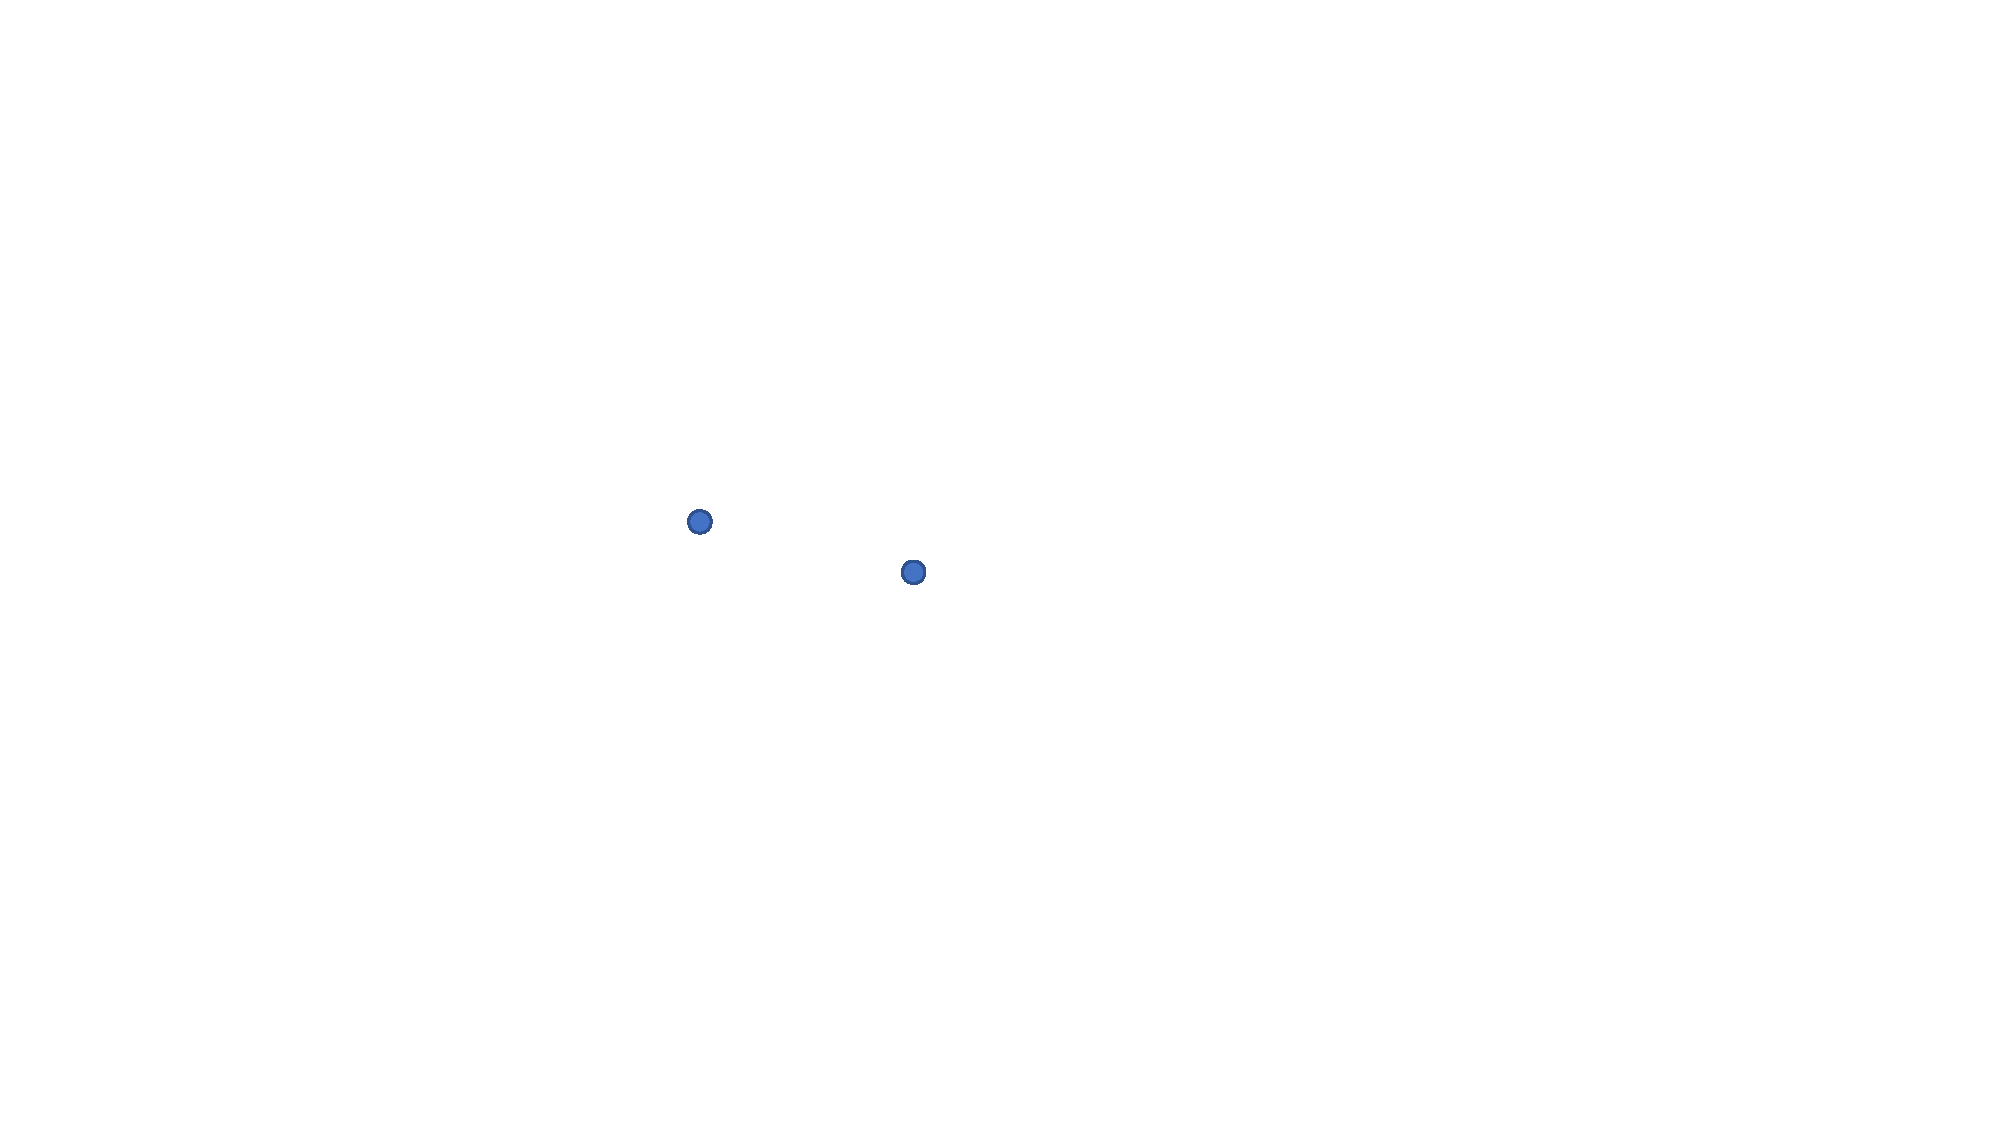
\includegraphics[width=0.425\linewidth]{../images/voronoi2.pdf}\hspace{10pt} \\
\hline
\hspace{10pt}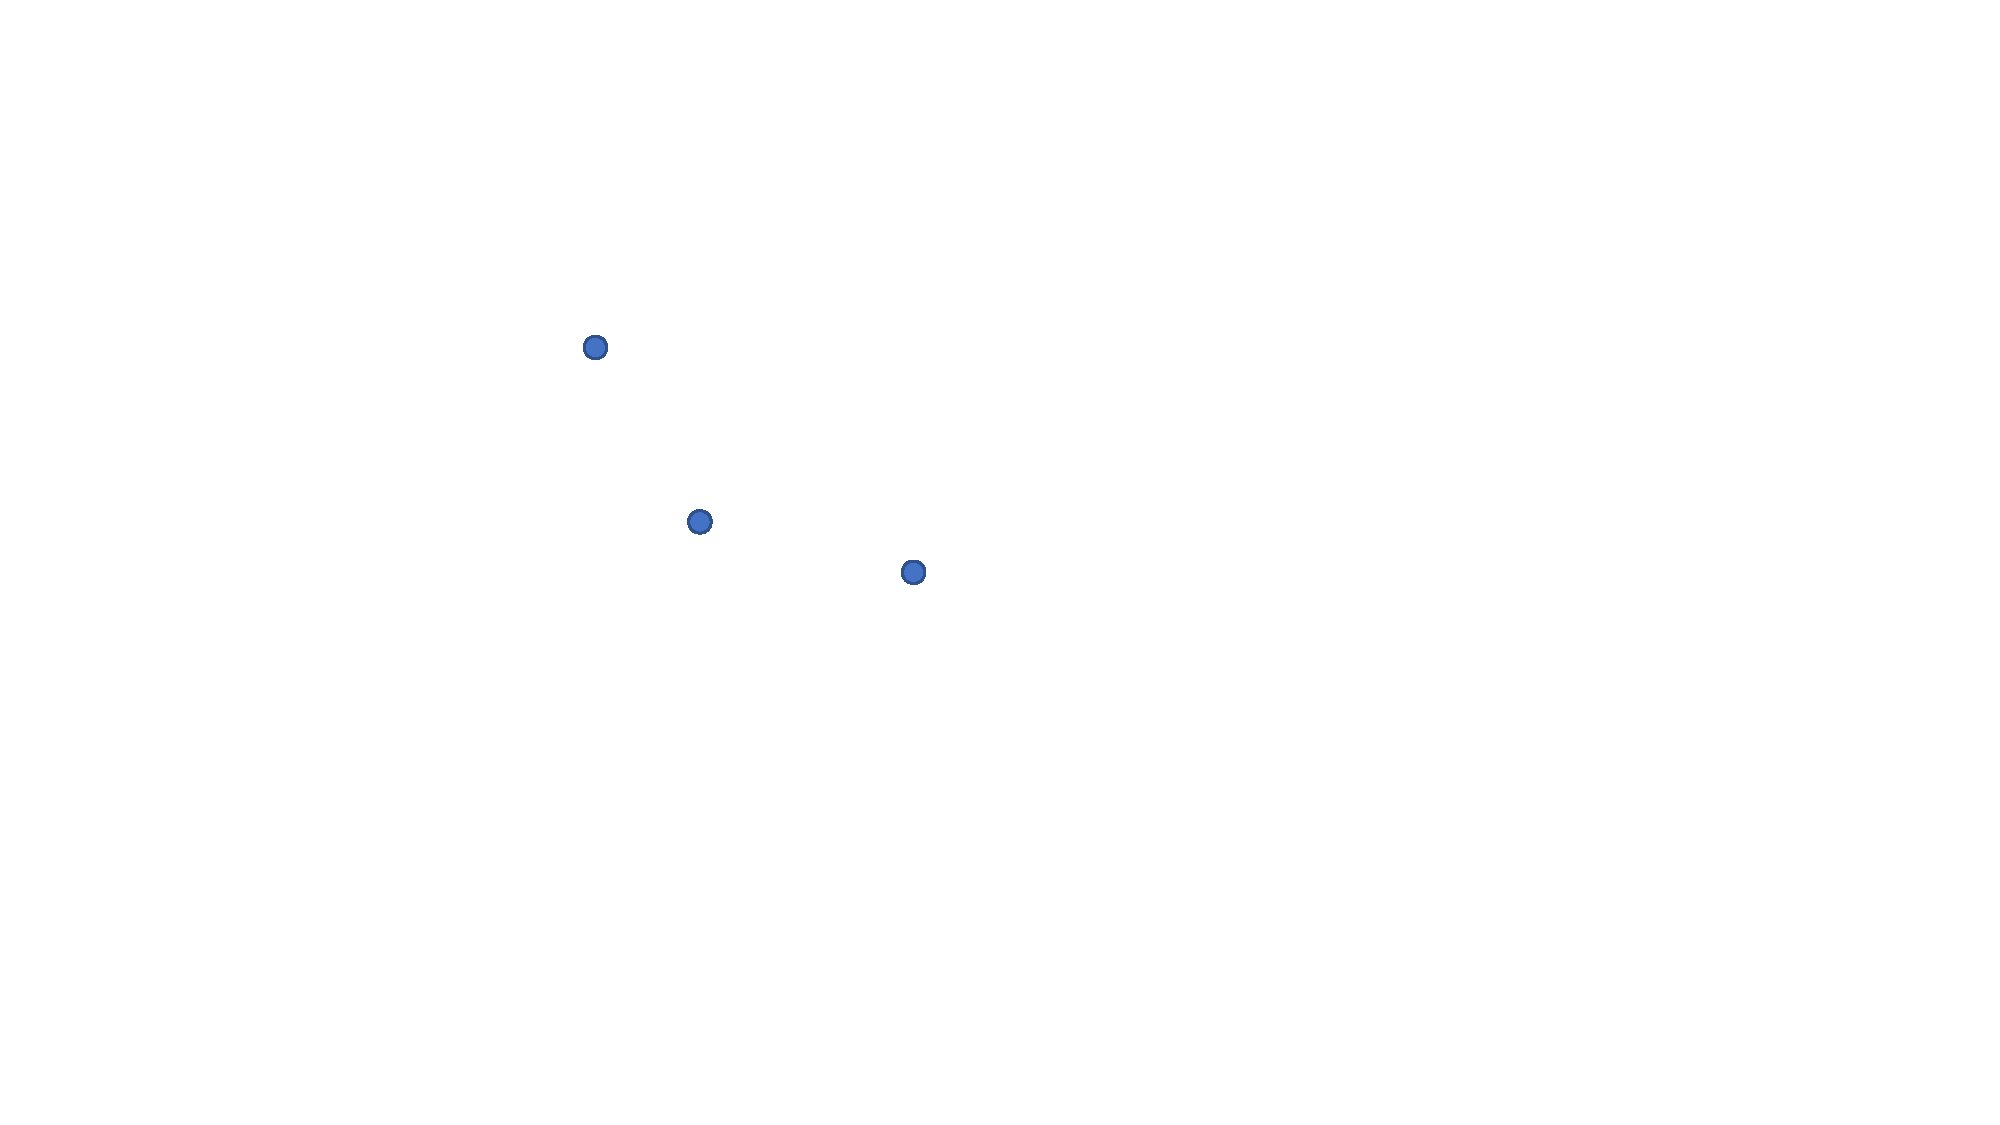
\includegraphics[width=0.425\linewidth]{../images/voronoi3.pdf}\hspace{10pt} & \hspace{10pt}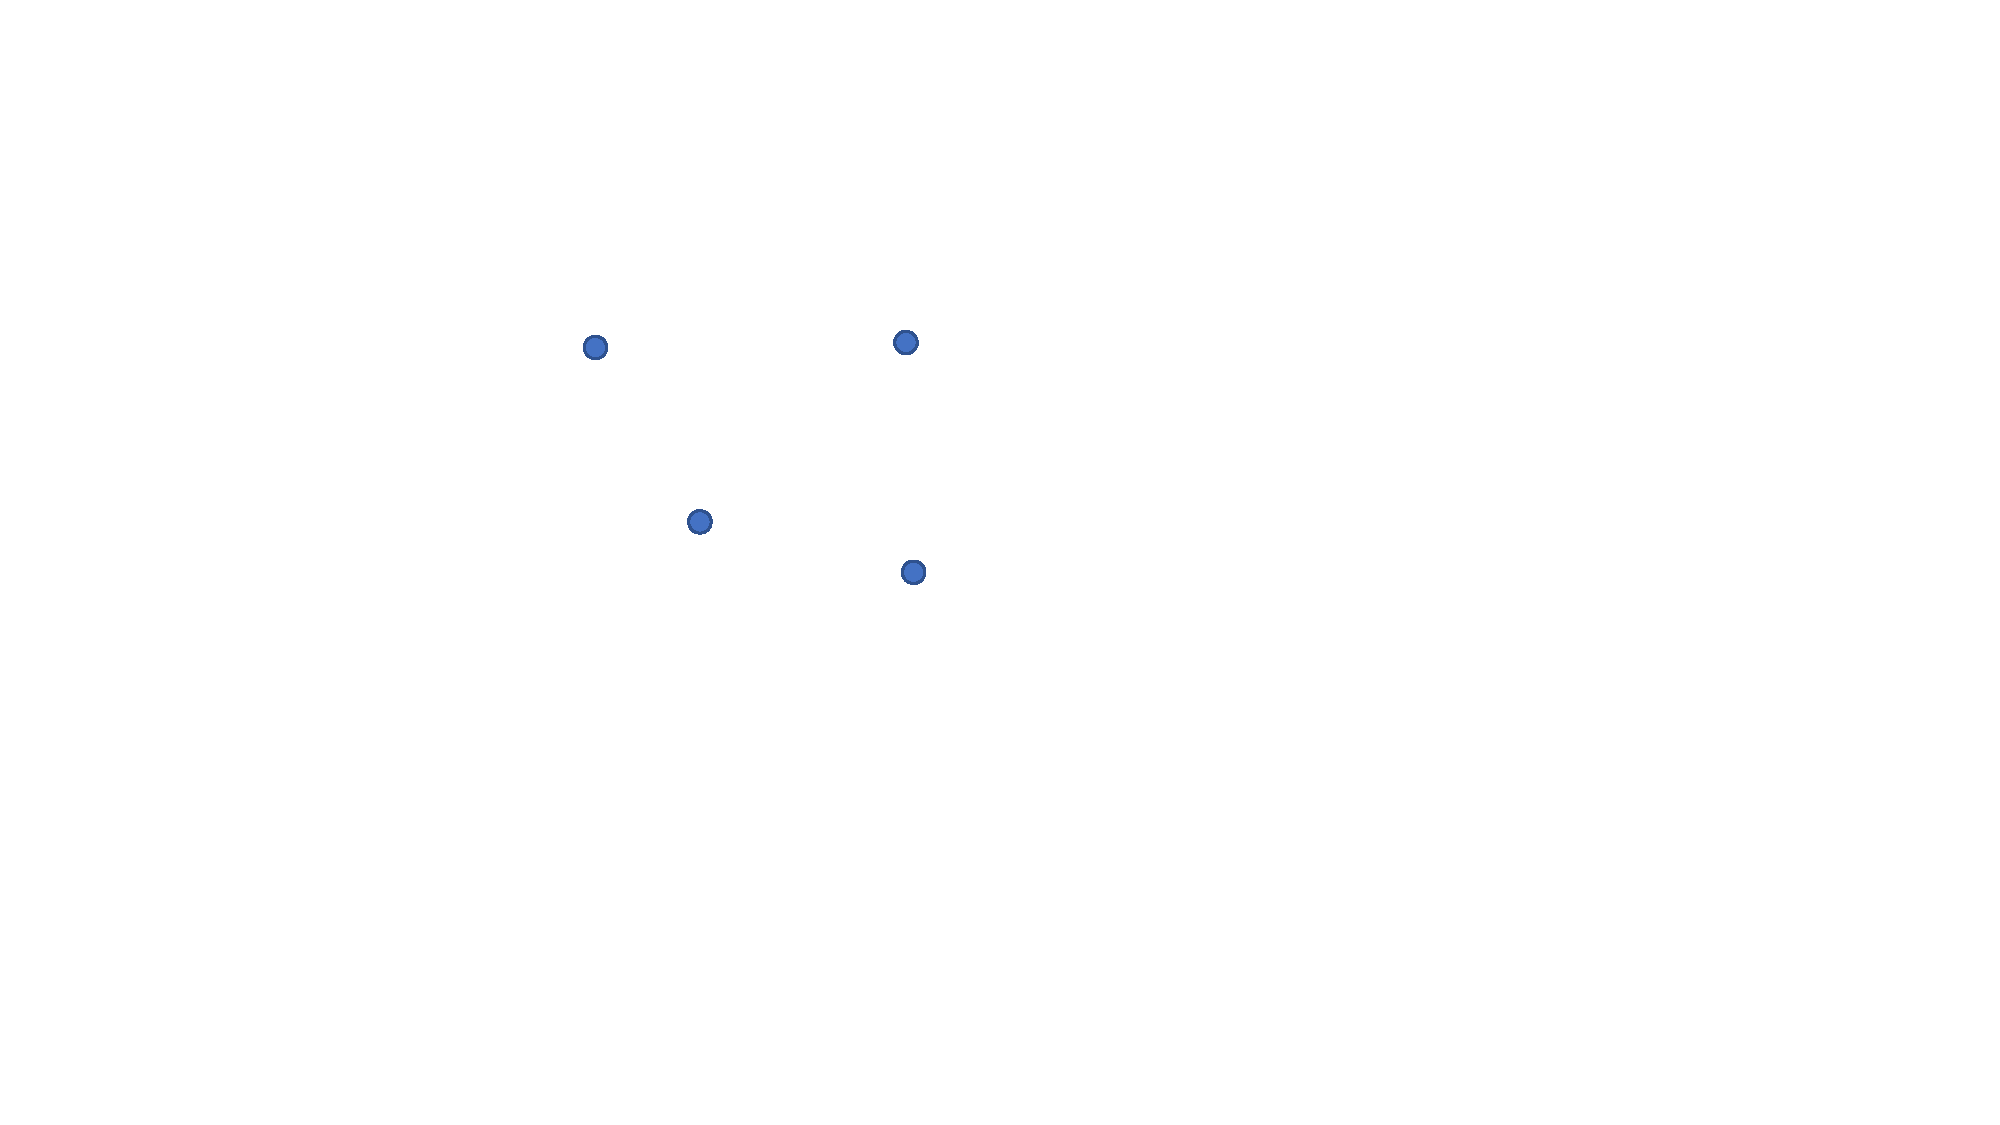
\includegraphics[width=0.425\linewidth]{../images/voronoi4.pdf}\hspace{10pt} \\
\hline
\end{tabular}

\begin{tabular}{|c|c|}
\hline
\hspace{10pt}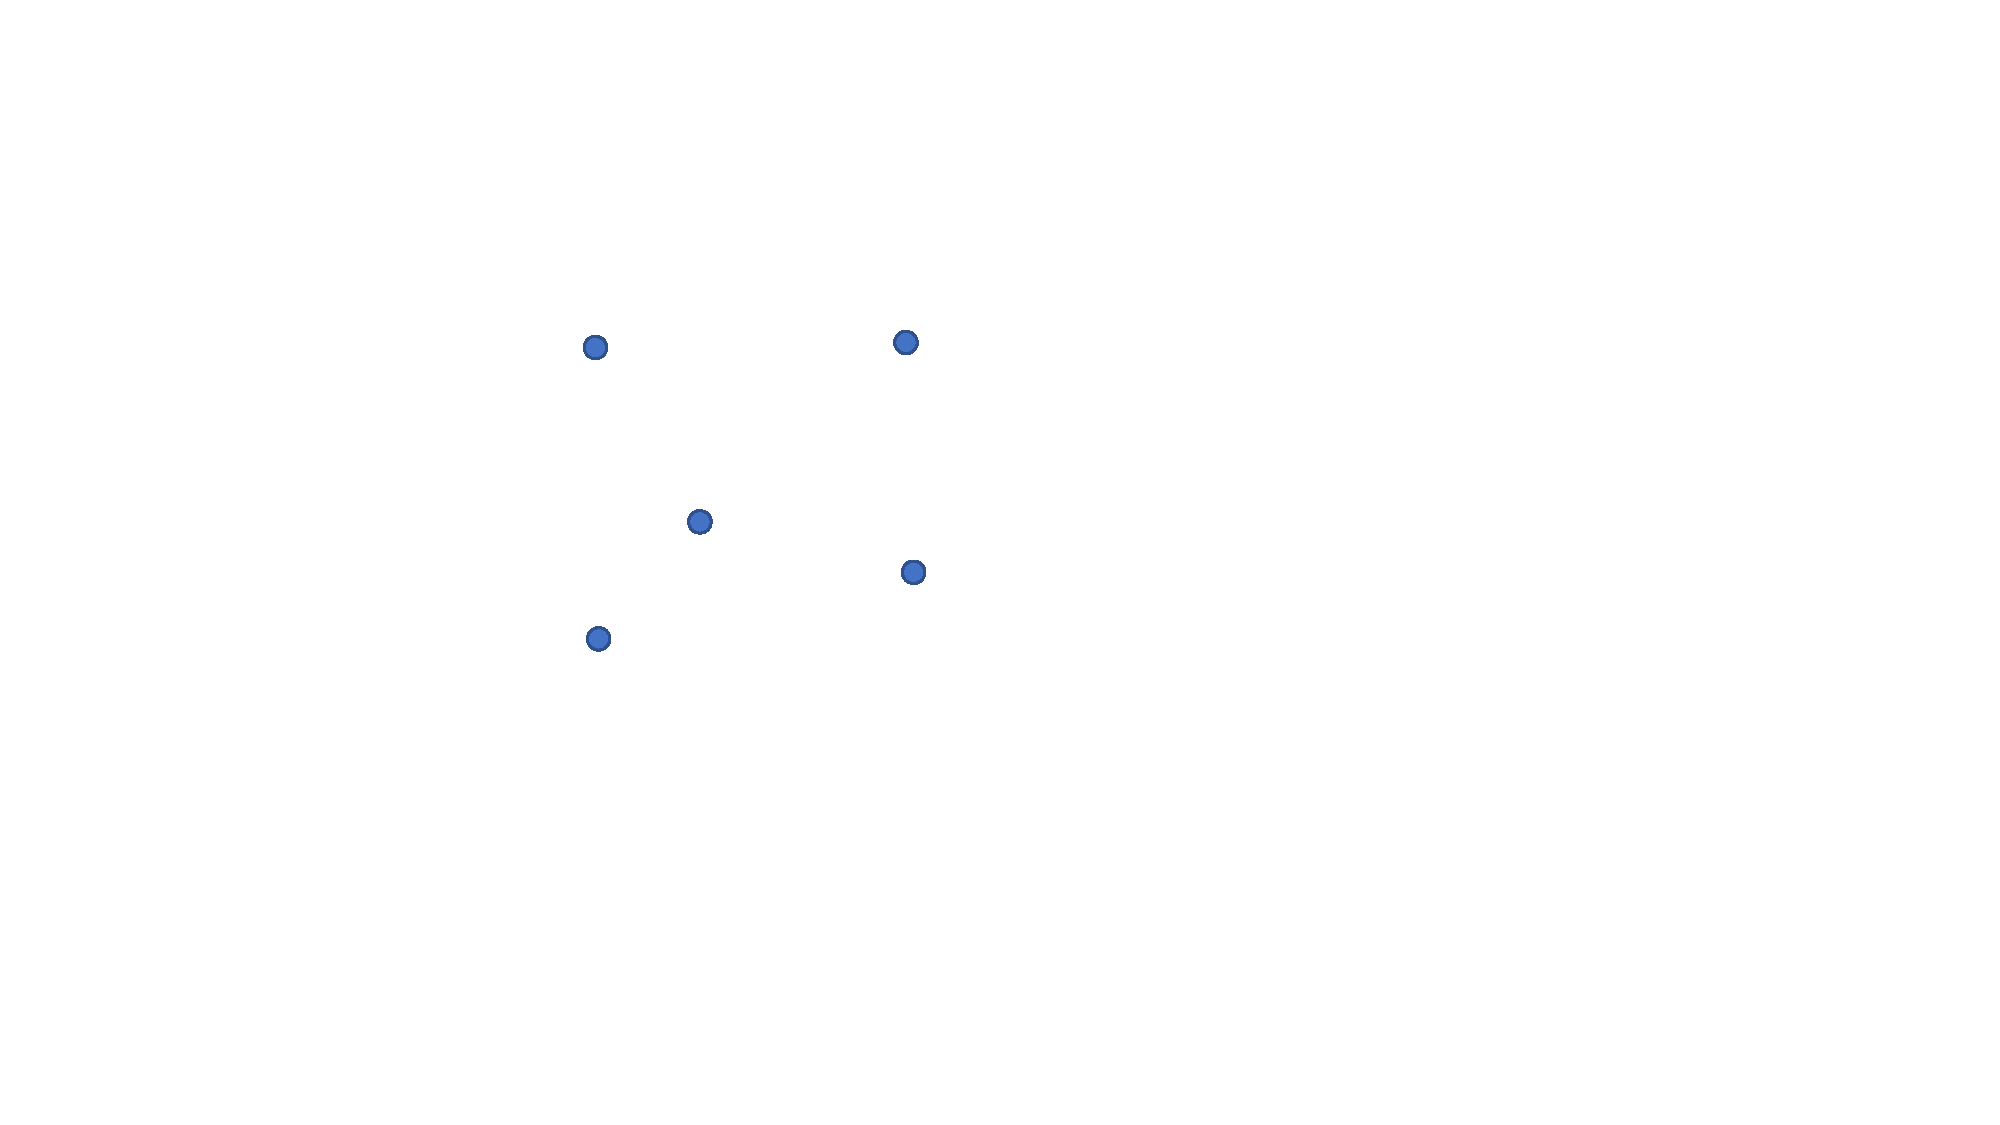
\includegraphics[width=0.425\linewidth]{../images/voronoi5.pdf}\hspace{10pt} & \hspace{10pt}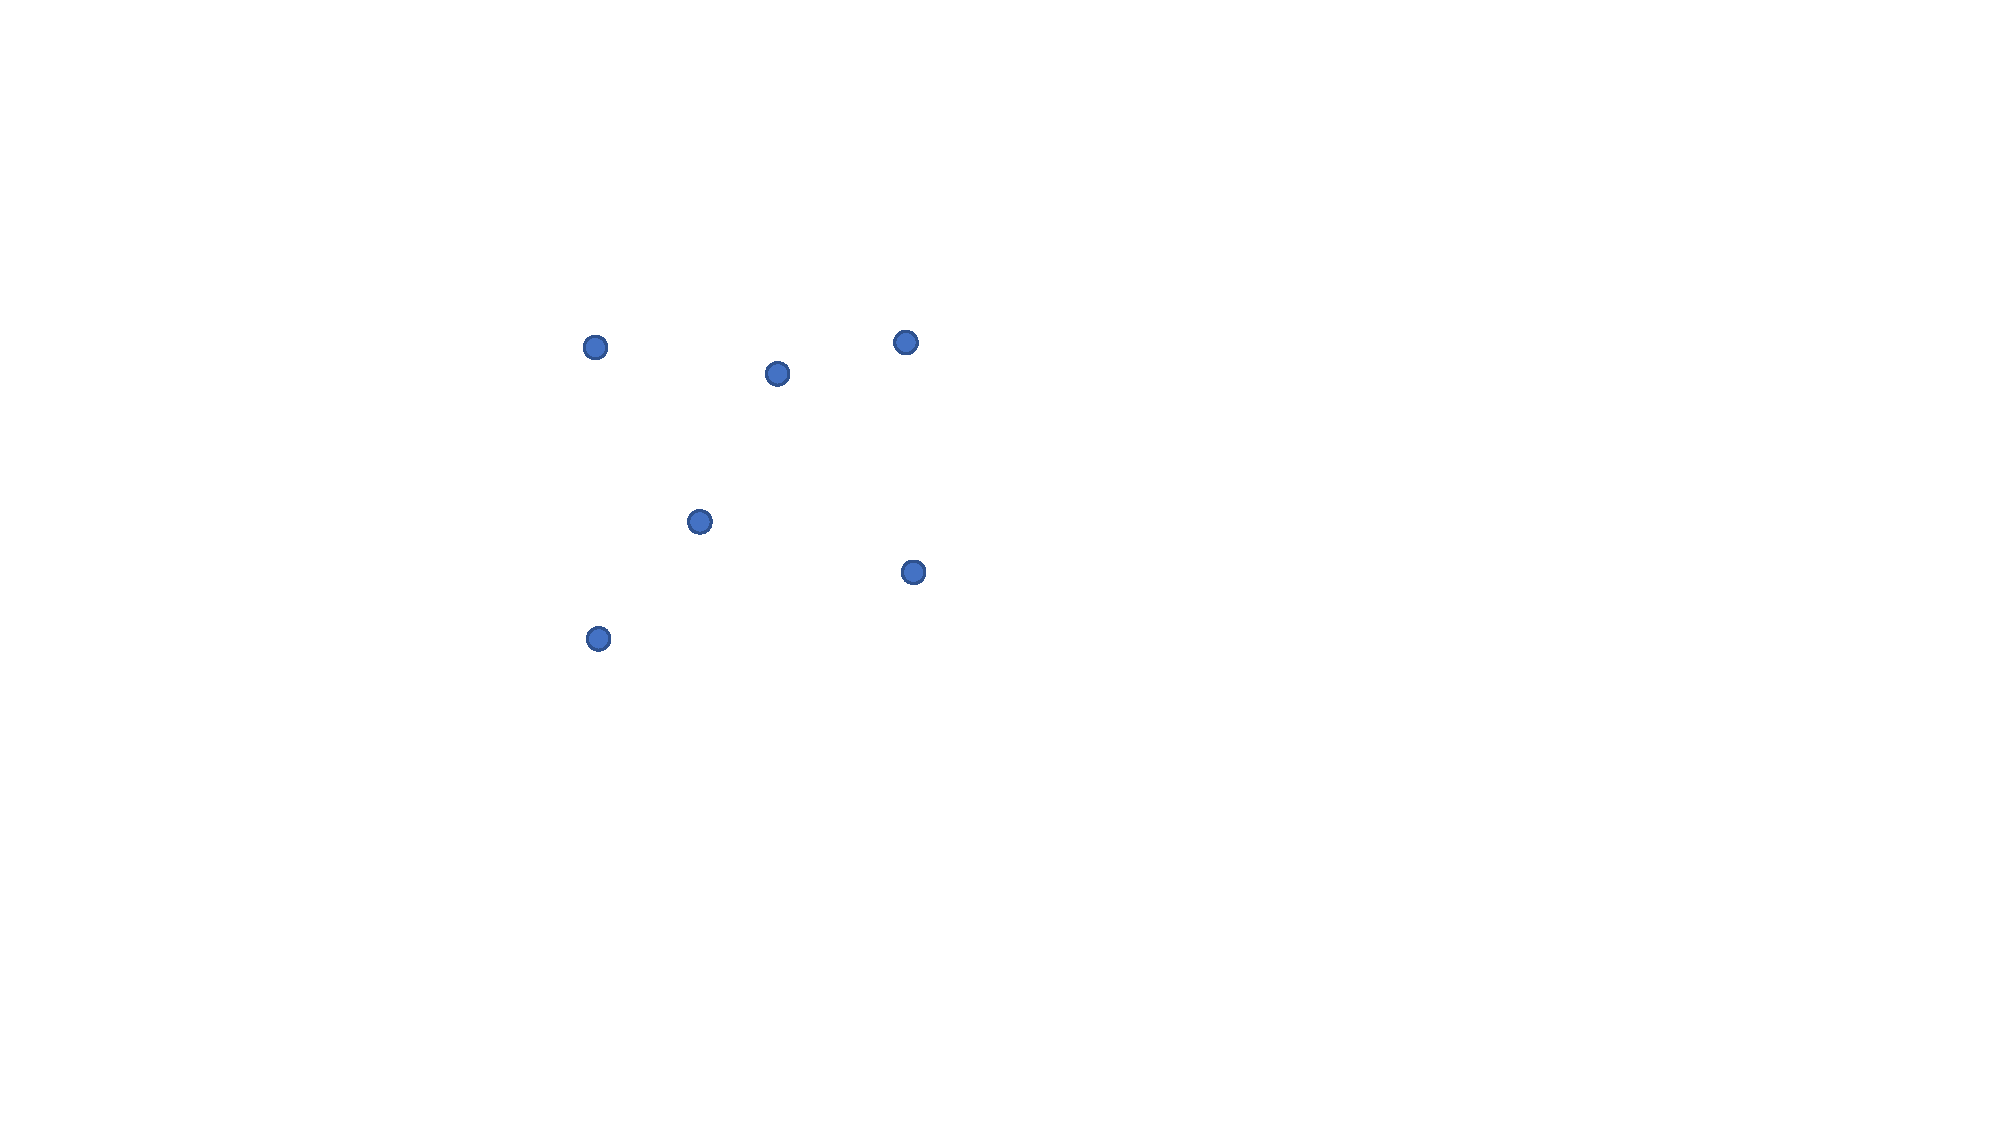
\includegraphics[width=0.425\linewidth]{../images/voronoi6.pdf}\hspace{10pt} \\
\hline
\hspace{10pt}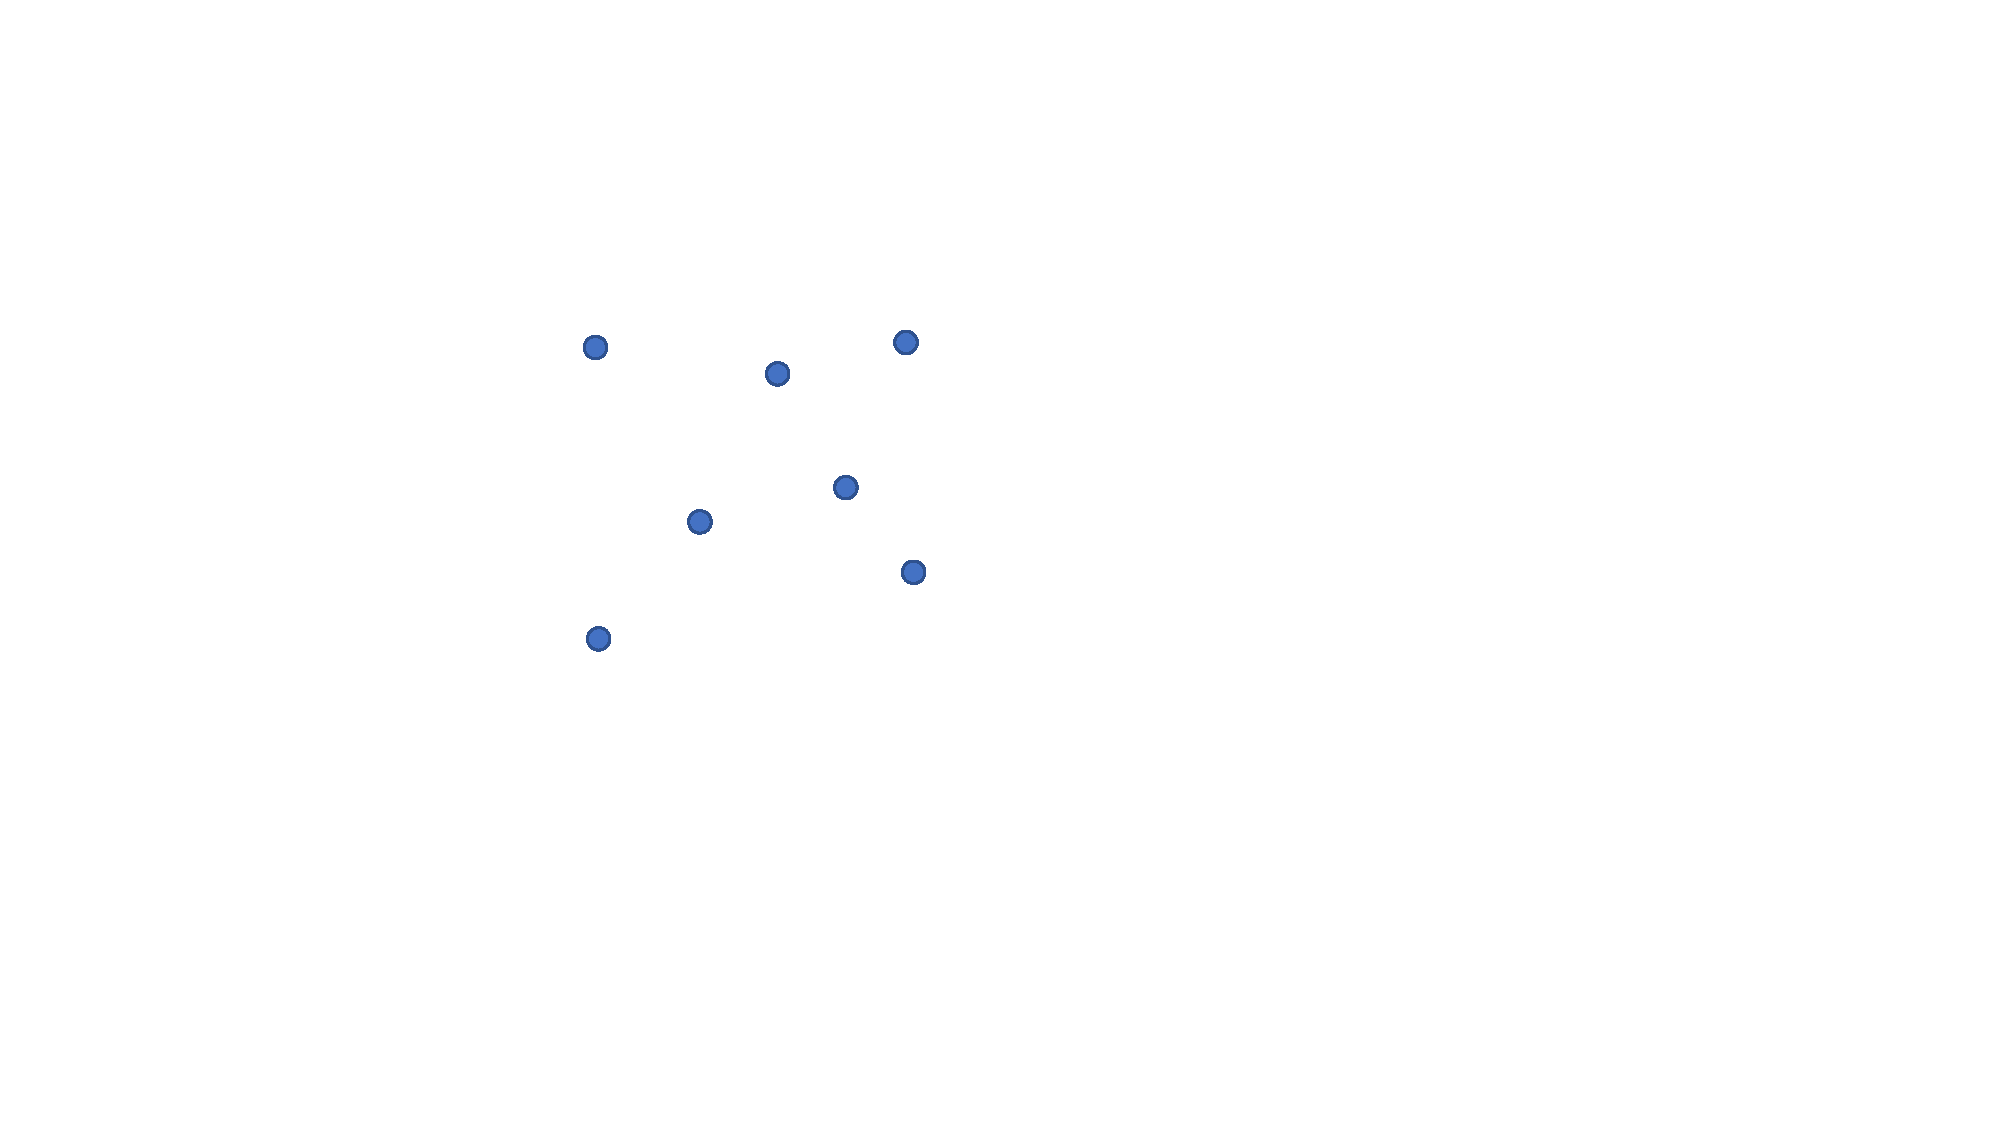
\includegraphics[width=0.425\linewidth]{../images/voronoi7.pdf}\hspace{10pt} \\
\cline{1-1}
\end{tabular}





\end{document}



